% Options for packages loaded elsewhere
% Options for packages loaded elsewhere
\PassOptionsToPackage{unicode}{hyperref}
\PassOptionsToPackage{hyphens}{url}
\PassOptionsToPackage{dvipsnames,svgnames,x11names}{xcolor}
%
\documentclass[
  custompaper,
  DIV=11,
  numbers=noendperiod]{scrartcl}
\usepackage{xcolor}
\usepackage{amsmath,amssymb}
\setcounter{secnumdepth}{-\maxdimen} % remove section numbering
\usepackage{iftex}
\ifPDFTeX
  \usepackage[T1]{fontenc}
  \usepackage[utf8]{inputenc}
  \usepackage{textcomp} % provide euro and other symbols
\else % if luatex or xetex
  \usepackage{unicode-math} % this also loads fontspec
  \defaultfontfeatures{Scale=MatchLowercase}
  \defaultfontfeatures[\rmfamily]{Ligatures=TeX,Scale=1}
\fi
\usepackage{lmodern}
\ifPDFTeX\else
  % xetex/luatex font selection
\fi
% Use upquote if available, for straight quotes in verbatim environments
\IfFileExists{upquote.sty}{\usepackage{upquote}}{}
\IfFileExists{microtype.sty}{% use microtype if available
  \usepackage[]{microtype}
  \UseMicrotypeSet[protrusion]{basicmath} % disable protrusion for tt fonts
}{}
\makeatletter
\@ifundefined{KOMAClassName}{% if non-KOMA class
  \IfFileExists{parskip.sty}{%
    \usepackage{parskip}
  }{% else
    \setlength{\parindent}{0pt}
    \setlength{\parskip}{6pt plus 2pt minus 1pt}}
}{% if KOMA class
  \KOMAoptions{parskip=half}}
\makeatother
% Make \paragraph and \subparagraph free-standing
\makeatletter
\ifx\paragraph\undefined\else
  \let\oldparagraph\paragraph
  \renewcommand{\paragraph}{
    \@ifstar
      \xxxParagraphStar
      \xxxParagraphNoStar
  }
  \newcommand{\xxxParagraphStar}[1]{\oldparagraph*{#1}\mbox{}}
  \newcommand{\xxxParagraphNoStar}[1]{\oldparagraph{#1}\mbox{}}
\fi
\ifx\subparagraph\undefined\else
  \let\oldsubparagraph\subparagraph
  \renewcommand{\subparagraph}{
    \@ifstar
      \xxxSubParagraphStar
      \xxxSubParagraphNoStar
  }
  \newcommand{\xxxSubParagraphStar}[1]{\oldsubparagraph*{#1}\mbox{}}
  \newcommand{\xxxSubParagraphNoStar}[1]{\oldsubparagraph{#1}\mbox{}}
\fi
\makeatother

\usepackage{color}
\usepackage{fancyvrb}
\newcommand{\VerbBar}{|}
\newcommand{\VERB}{\Verb[commandchars=\\\{\}]}
\DefineVerbatimEnvironment{Highlighting}{Verbatim}{commandchars=\\\{\}}
% Add ',fontsize=\small' for more characters per line
\usepackage{framed}
\definecolor{shadecolor}{RGB}{241,243,245}
\newenvironment{Shaded}{\begin{snugshade}}{\end{snugshade}}
\newcommand{\AlertTok}[1]{\textcolor[rgb]{0.68,0.00,0.00}{#1}}
\newcommand{\AnnotationTok}[1]{\textcolor[rgb]{0.37,0.37,0.37}{#1}}
\newcommand{\AttributeTok}[1]{\textcolor[rgb]{0.40,0.45,0.13}{#1}}
\newcommand{\BaseNTok}[1]{\textcolor[rgb]{0.68,0.00,0.00}{#1}}
\newcommand{\BuiltInTok}[1]{\textcolor[rgb]{0.00,0.23,0.31}{#1}}
\newcommand{\CharTok}[1]{\textcolor[rgb]{0.13,0.47,0.30}{#1}}
\newcommand{\CommentTok}[1]{\textcolor[rgb]{0.37,0.37,0.37}{#1}}
\newcommand{\CommentVarTok}[1]{\textcolor[rgb]{0.37,0.37,0.37}{\textit{#1}}}
\newcommand{\ConstantTok}[1]{\textcolor[rgb]{0.56,0.35,0.01}{#1}}
\newcommand{\ControlFlowTok}[1]{\textcolor[rgb]{0.00,0.23,0.31}{\textbf{#1}}}
\newcommand{\DataTypeTok}[1]{\textcolor[rgb]{0.68,0.00,0.00}{#1}}
\newcommand{\DecValTok}[1]{\textcolor[rgb]{0.68,0.00,0.00}{#1}}
\newcommand{\DocumentationTok}[1]{\textcolor[rgb]{0.37,0.37,0.37}{\textit{#1}}}
\newcommand{\ErrorTok}[1]{\textcolor[rgb]{0.68,0.00,0.00}{#1}}
\newcommand{\ExtensionTok}[1]{\textcolor[rgb]{0.00,0.23,0.31}{#1}}
\newcommand{\FloatTok}[1]{\textcolor[rgb]{0.68,0.00,0.00}{#1}}
\newcommand{\FunctionTok}[1]{\textcolor[rgb]{0.28,0.35,0.67}{#1}}
\newcommand{\ImportTok}[1]{\textcolor[rgb]{0.00,0.46,0.62}{#1}}
\newcommand{\InformationTok}[1]{\textcolor[rgb]{0.37,0.37,0.37}{#1}}
\newcommand{\KeywordTok}[1]{\textcolor[rgb]{0.00,0.23,0.31}{\textbf{#1}}}
\newcommand{\NormalTok}[1]{\textcolor[rgb]{0.00,0.23,0.31}{#1}}
\newcommand{\OperatorTok}[1]{\textcolor[rgb]{0.37,0.37,0.37}{#1}}
\newcommand{\OtherTok}[1]{\textcolor[rgb]{0.00,0.23,0.31}{#1}}
\newcommand{\PreprocessorTok}[1]{\textcolor[rgb]{0.68,0.00,0.00}{#1}}
\newcommand{\RegionMarkerTok}[1]{\textcolor[rgb]{0.00,0.23,0.31}{#1}}
\newcommand{\SpecialCharTok}[1]{\textcolor[rgb]{0.37,0.37,0.37}{#1}}
\newcommand{\SpecialStringTok}[1]{\textcolor[rgb]{0.13,0.47,0.30}{#1}}
\newcommand{\StringTok}[1]{\textcolor[rgb]{0.13,0.47,0.30}{#1}}
\newcommand{\VariableTok}[1]{\textcolor[rgb]{0.07,0.07,0.07}{#1}}
\newcommand{\VerbatimStringTok}[1]{\textcolor[rgb]{0.13,0.47,0.30}{#1}}
\newcommand{\WarningTok}[1]{\textcolor[rgb]{0.37,0.37,0.37}{\textit{#1}}}

\usepackage{longtable,booktabs,array}
\usepackage{calc} % for calculating minipage widths
% Correct order of tables after \paragraph or \subparagraph
\usepackage{etoolbox}
\makeatletter
\patchcmd\longtable{\par}{\if@noskipsec\mbox{}\fi\par}{}{}
\makeatother
% Allow footnotes in longtable head/foot
\IfFileExists{footnotehyper.sty}{\usepackage{footnotehyper}}{\usepackage{footnote}}
\makesavenoteenv{longtable}
\usepackage{graphicx}
\makeatletter
\newsavebox\pandoc@box
\newcommand*\pandocbounded[1]{% scales image to fit in text height/width
  \sbox\pandoc@box{#1}%
  \Gscale@div\@tempa{\textheight}{\dimexpr\ht\pandoc@box+\dp\pandoc@box\relax}%
  \Gscale@div\@tempb{\linewidth}{\wd\pandoc@box}%
  \ifdim\@tempb\p@<\@tempa\p@\let\@tempa\@tempb\fi% select the smaller of both
  \ifdim\@tempa\p@<\p@\scalebox{\@tempa}{\usebox\pandoc@box}%
  \else\usebox{\pandoc@box}%
  \fi%
}
% Set default figure placement to htbp
\def\fps@figure{htbp}
\makeatother





\setlength{\emergencystretch}{3em} % prevent overfull lines

\providecommand{\tightlist}{%
  \setlength{\itemsep}{0pt}\setlength{\parskip}{0pt}}



 


\KOMAoption{captions}{tableheading}
\makeatletter
\@ifpackageloaded{caption}{}{\usepackage{caption}}
\AtBeginDocument{%
\ifdefined\contentsname
  \renewcommand*\contentsname{Table of contents}
\else
  \newcommand\contentsname{Table of contents}
\fi
\ifdefined\listfigurename
  \renewcommand*\listfigurename{List of Figures}
\else
  \newcommand\listfigurename{List of Figures}
\fi
\ifdefined\listtablename
  \renewcommand*\listtablename{List of Tables}
\else
  \newcommand\listtablename{List of Tables}
\fi
\ifdefined\figurename
  \renewcommand*\figurename{Figure}
\else
  \newcommand\figurename{Figure}
\fi
\ifdefined\tablename
  \renewcommand*\tablename{Table}
\else
  \newcommand\tablename{Table}
\fi
}
\@ifpackageloaded{float}{}{\usepackage{float}}
\floatstyle{ruled}
\@ifundefined{c@chapter}{\newfloat{codelisting}{h}{lop}}{\newfloat{codelisting}{h}{lop}[chapter]}
\floatname{codelisting}{Listing}
\newcommand*\listoflistings{\listof{codelisting}{List of Listings}}
\makeatother
\makeatletter
\makeatother
\makeatletter
\@ifpackageloaded{caption}{}{\usepackage{caption}}
\@ifpackageloaded{subcaption}{}{\usepackage{subcaption}}
\makeatother
\makeatletter
\@ifpackageloaded{fontawesome6}{}{\usepackage{fontawesome6}}
\makeatother
\usepackage{bookmark}
\IfFileExists{xurl.sty}{\usepackage{xurl}}{} % add URL line breaks if available
\urlstyle{same}
\hypersetup{
  pdftitle={Quantitative Methoden mit R \& R-Studio},
  pdfauthor={Maura Kratz},
  colorlinks=true,
  linkcolor={blue},
  filecolor={Maroon},
  citecolor={Blue},
  urlcolor={Blue},
  pdfcreator={LaTeX via pandoc}}


\title{Quantitative Methoden mit R \& R-Studio}
\usepackage{etoolbox}
\makeatletter
\providecommand{\subtitle}[1]{% add subtitle to \maketitle
  \apptocmd{\@title}{\par {\large #1 \par}}{}{}
}
\makeatother
\subtitle{Sommersemester 2026 \textbar{} Sitzung 3}
\author{Maura Kratz}
\date{}
\begin{document}
\maketitle


\subsection{Willkommen zurück!}\label{willkommen-zuruxfcck}

\pandocbounded{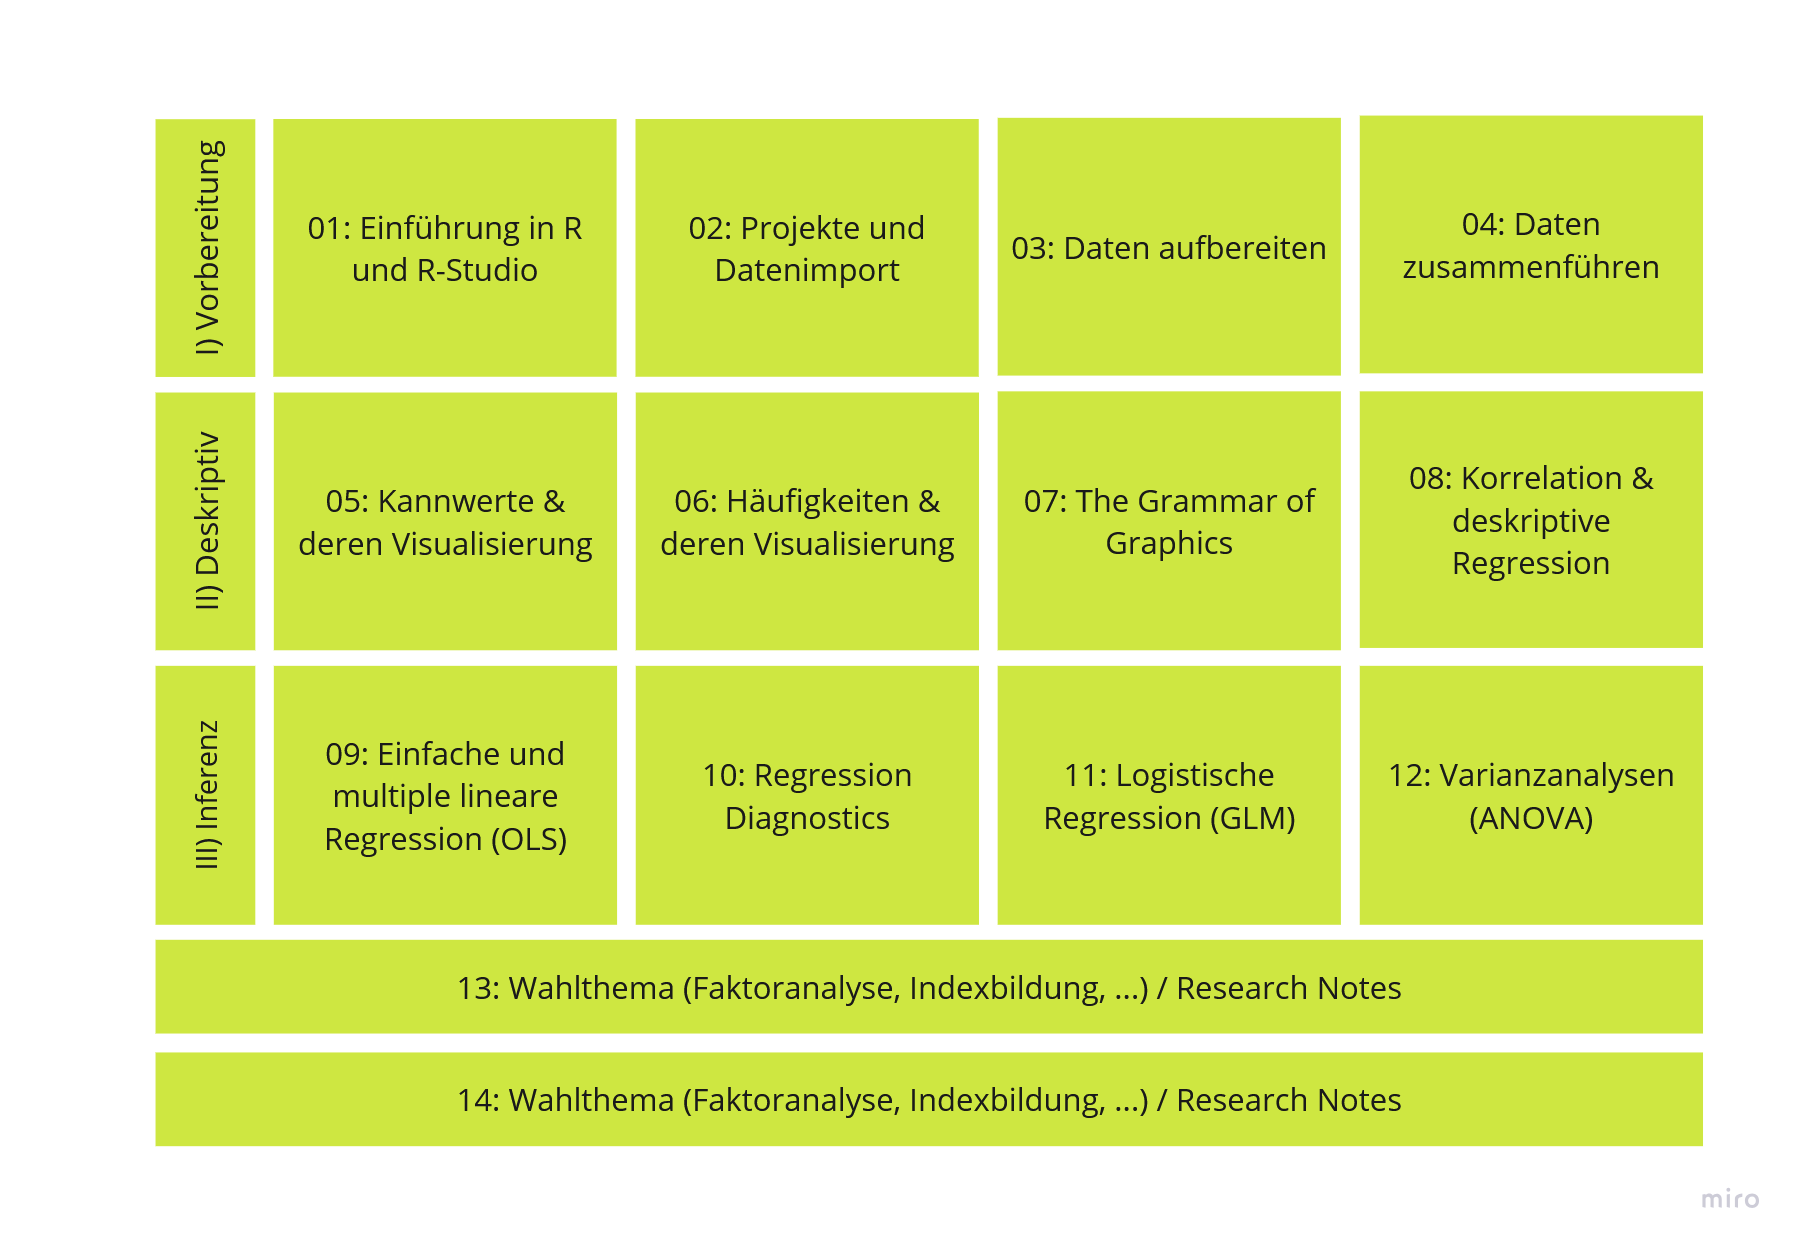
\includegraphics[keepaspectratio]{images/clipboard-4994590.png}}

\section{Was heute ansteht:}\label{was-heute-ansteht}

\begin{itemize}
\tightlist
\item
  Check-In
\item
  Besprechung der Übung 1
\item
  Data Cleaning \& Wrangling
\end{itemize}

\section{Recap}\label{recap}

\begin{enumerate}
\def\labelenumi{\arabic{enumi}.}
\tightlist
\item
  Projektordner anlegen und darin arbeiten \faIcon{check}
\item
  tidy code und tidy Kommentare schreiben \faIcon{check}
\item
  Hilfe suchen \faIcon{check}
\item
  Daten einlesen mit dem \emph{rio}-Paket \faIcon{check}
\item
  Daten überblicken mit dem \emph{summarytools}-Paket \faIcon{check}
\end{enumerate}

\subsection{Datenanalyse-Workflow}\label{datenanalyse-workflow}

\pandocbounded{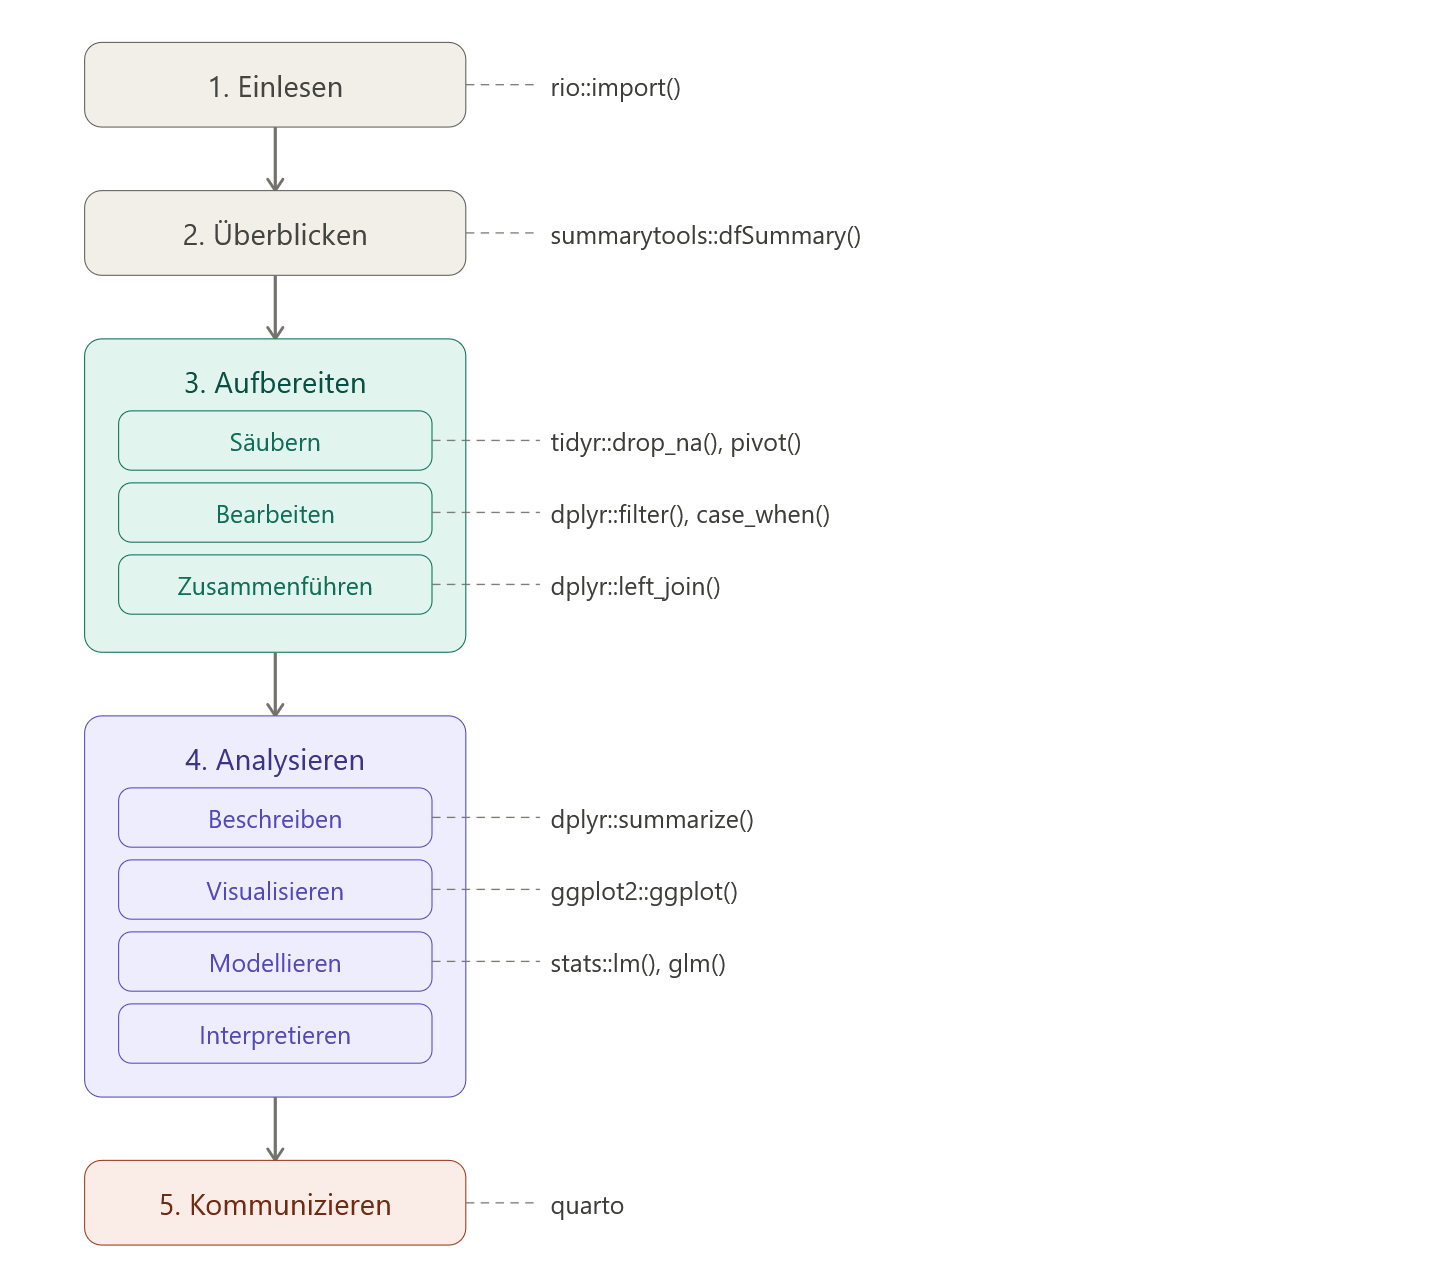
\includegraphics[keepaspectratio]{images/clipboard-4263712504.png}}

\subsection{Pakete}\label{pakete}

\begin{itemize}
\tightlist
\item
  Einige Funktionen sind bereits in base R enthalten
\item
  Für andere müssen zusätzliche Pakete geladen werden
\item
  Pakete sind Bündel unterschiedlicher Funktionen
\item
  Base R reicht oft nur für sehr basale Operationen und
  Visualisierungen, für alles andere werden Pakete benötigt
\end{itemize}

\pandocbounded{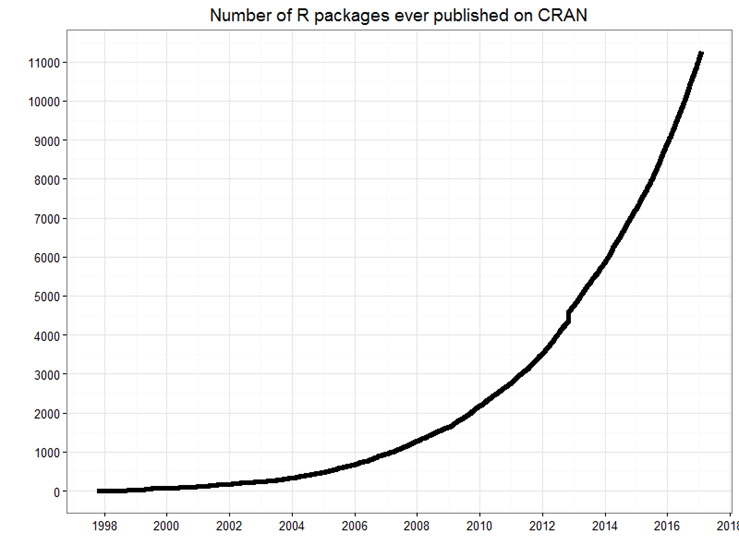
\includegraphics[keepaspectratio]{images/clipboard-2773888020.png}}

\subsection{\texorpdfstring{\emph{summarytools}-Paket}{summarytools-Paket}}\label{summarytools-paket}

\begin{longtable}[]{@{}
  >{\raggedright\arraybackslash}p{(\linewidth - 4\tabcolsep) * \real{0.3333}}
  >{\raggedright\arraybackslash}p{(\linewidth - 4\tabcolsep) * \real{0.3333}}
  >{\raggedright\arraybackslash}p{(\linewidth - 4\tabcolsep) * \real{0.3333}}@{}}
\toprule\noalign{}
\begin{minipage}[b]{\linewidth}\raggedright
Funktion
\end{minipage} & \begin{minipage}[b]{\linewidth}\raggedright
Beschreibung
\end{minipage} & \begin{minipage}[b]{\linewidth}\raggedright
Geeignet für
\end{minipage} \\
\midrule\noalign{}
\endhead
\bottomrule\noalign{}
\endlastfoot
\texttt{dfSummary()} & Übersicht über alle Variablen (Klasse, fehlende
Werte, Verteilungen, etc.) & Schnelle Gesamtübersicht eines
Datensatzes \\
\texttt{freq()} & Häufigkeitstabellen & Einfache Verteilungen
kategorialer Variablen \\
\texttt{descr()} & Deskriptive Statistik (Mittelwert, Median, SD, etc.)
& Basisanalyse numerischer Variablen \\
\texttt{ctable()} & Kreuztabellen mit Prozenten und optionalen Tests (z.
B. Chi²) & Zusammenhang zwischen zweikategorialen Variablen \\
\end{longtable}

\begin{Shaded}
\begin{Highlighting}[]
\NormalTok{btw\_2025\_ergebnisse }\SpecialCharTok{\%\textgreater{}\%}
\NormalTok{  summarytools}\SpecialCharTok{::}\FunctionTok{dfSummary}\NormalTok{(}\AttributeTok{na.col =} \ConstantTok{FALSE}\NormalTok{) }\SpecialCharTok{\%\textgreater{}\%} \CommentTok{\# missings{-}Spalte ausblenden}
\NormalTok{  summarytools}\SpecialCharTok{::}\FunctionTok{view}\NormalTok{(}\AttributeTok{file =} \StringTok{"./data/btw\_2025\_ergebnisse\_uebersicht.html"}\NormalTok{) }\CommentTok{\# speichern}
\end{Highlighting}
\end{Shaded}

\section{\texorpdfstring{Das
\emph{tidyverse}-Paketbündel}{Das tidyverse-Paketbündel}}\label{das-tidyverse-paketbuxfcndel}

\pandocbounded{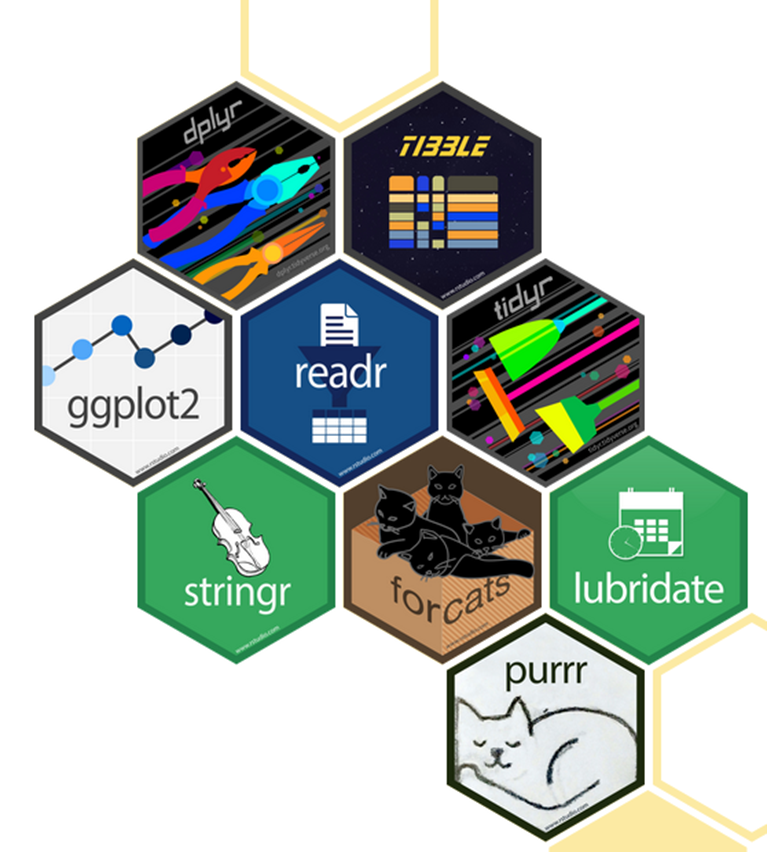
\includegraphics[keepaspectratio]{images/clipboard-199054296.png}}

\subsection{Pipes}\label{pipes}

\begin{itemize}
\tightlist
\item
  Zwei Optionen: Base R pipe: \texttt{\textbar{}\textgreater{}} ODER
  magrittr pipe: \texttt{\%\textgreater{}\%}
\item
  Die Default-Pipe kann über \emph{Global Options} eingestellt werden
\item
  Zum Einfügen: eintippen oder \texttt{Strg\ +\ Shift\ +\ M}
\item
  Stilregeln:

  \begin{itemize}
  \tightlist
  \item
    Immer Leerzeichen vor der Pipe
  \item
    Immer neue Zeile danach
  \end{itemize}
\end{itemize}

\begin{Shaded}
\begin{Highlighting}[]
\NormalTok{btw\_2025\_ergebnisse }\SpecialCharTok{\%\textgreater{}\%}
\NormalTok{  dplyr}\SpecialCharTok{::}\FunctionTok{filter}\NormalTok{(jahr }\SpecialCharTok{==} \DecValTok{2025}\NormalTok{) }\SpecialCharTok{\%\textgreater{}\%}
\NormalTok{  dplyr}\SpecialCharTok{::}\FunctionTok{select}\NormalTok{(partei, zweitstimmen)}
\end{Highlighting}
\end{Shaded}

\section{Hands On - Data Wrangling}\label{hands-on---data-wrangling}

\pandocbounded{
\includegraphics[keepaspectratio]{images/clipboard-797395825.jpeg}}

\subsection{\texorpdfstring{Datentransformation mit
\emph{dplyr}}{Datentransformation mit dplyr}}\label{datentransformation-mit-dplyr}

\begin{longtable}[]{@{}
  >{\raggedright\arraybackslash}p{(\linewidth - 4\tabcolsep) * \real{0.3333}}
  >{\raggedright\arraybackslash}p{(\linewidth - 4\tabcolsep) * \real{0.3333}}
  >{\raggedright\arraybackslash}p{(\linewidth - 4\tabcolsep) * \real{0.3333}}@{}}
\toprule\noalign{}
\begin{minipage}[b]{\linewidth}\raggedright
Befehl
\end{minipage} & \begin{minipage}[b]{\linewidth}\raggedright
Beschreibung
\end{minipage} & \begin{minipage}[b]{\linewidth}\raggedright
Bsp
\end{minipage} \\
\midrule\noalign{}
\endhead
\bottomrule\noalign{}
\endlastfoot
\texttt{rename()} & Spaltennamen ändern &
\texttt{df\ \%\textgreater{}\%\ rename(neu\ =\ alt)} \\
\texttt{select()} & Variablen auswählen &
\texttt{df\ \%\textgreater{}\%\ select(var1,\ var2)} \\
\texttt{slice()} & Zeilen nach Position auswählen &
\texttt{df\ \%\textgreater{}\%\ slice(1:10)} \\
\texttt{filter()} & Zeilen nach Werten filtern &
\texttt{df\ \%\textgreater{}\%\ filter(jahr\ ==\ 2025)} \\
\texttt{relocate()} & Spaltenreihenfolge ändern &
\texttt{df\ \%\textgreater{}\%\ relocate(var1,\ .before\ =\ var2)} \\
\end{longtable}

\subsection{\texorpdfstring{Datentransformation mit mit
\emph{dplyr}}{Datentransformation mit mit dplyr}}\label{datentransformation-mit-mit-dplyr}

\begin{longtable}[]{@{}
  >{\raggedright\arraybackslash}p{(\linewidth - 4\tabcolsep) * \real{0.3333}}
  >{\raggedright\arraybackslash}p{(\linewidth - 4\tabcolsep) * \real{0.3333}}
  >{\raggedright\arraybackslash}p{(\linewidth - 4\tabcolsep) * \real{0.3333}}@{}}
\toprule\noalign{}
\begin{minipage}[b]{\linewidth}\raggedright
Befehl
\end{minipage} & \begin{minipage}[b]{\linewidth}\raggedright
Beschreibung
\end{minipage} & \begin{minipage}[b]{\linewidth}\raggedright
Bsp
\end{minipage} \\
\midrule\noalign{}
\endhead
\bottomrule\noalign{}
\endlastfoot
\texttt{mutate()} & Neue Variablen hinzufügen &
\texttt{df\ \%\textgreater{}\%\ mutate(anteil\ =\ stimmen\ /\ sum(stimmen))} \\
\texttt{summarise()} & Mehrere Werte zusammenfassen &
\texttt{df\ \%\textgreater{}\%\ summarise(mean(stimmen))} \\
\texttt{count()} & Häufigkeiten zählen &
\texttt{df\ \%\textgreater{}\%\ count(partei)} \\
\texttt{group\_by()} & Operationen gruppenweise ausführen &
\texttt{df\ \%\textgreater{}\%\ group\_by(partei)\ \%\textgreater{}\%\ summarise(mean(stimmen))} \\
\end{longtable}

\subsection{\texorpdfstring{Datentransformation mit mit
\emph{tidyr}}{Datentransformation mit mit tidyr}}\label{datentransformation-mit-mit-tidyr}

\begin{longtable}[]{@{}
  >{\raggedright\arraybackslash}p{(\linewidth - 4\tabcolsep) * \real{0.3333}}
  >{\raggedright\arraybackslash}p{(\linewidth - 4\tabcolsep) * \real{0.3333}}
  >{\raggedright\arraybackslash}p{(\linewidth - 4\tabcolsep) * \real{0.3333}}@{}}
\toprule\noalign{}
\begin{minipage}[b]{\linewidth}\raggedright
Befehl
\end{minipage} & \begin{minipage}[b]{\linewidth}\raggedright
Beschreibung
\end{minipage} & \begin{minipage}[b]{\linewidth}\raggedright
Bsp
\end{minipage} \\
\midrule\noalign{}
\endhead
\bottomrule\noalign{}
\endlastfoot
\texttt{pivot\_longer()} & Breites Format in langes umwandeln &
\texttt{df\ \%\textgreater{}\%\ pivot\_longer(cols\ =\ -id,\ names\_to\ =\ "var",\ values\_to\ =\ "val")} \\
\texttt{pivot\_wider()} & Langes Format in breites umwandeln &
\texttt{df\ \%\textgreater{}\%\ pivot\_wider(names\_from\ =\ var,\ values\_from\ =\ val)} \\
\texttt{drop\_na()} & Zeilen mit fehlenden Werten entfernen &
\texttt{df\ \%\textgreater{}\%\ drop\_na(var1)} \\
\end{longtable}

\subsection{Änderungen überprüfen - 3
Optionen}\label{uxe4nderungen-uxfcberpruxfcfen---3-optionen}

\textbf{1. In der Console ansehen}

\begin{itemize}
\item
  Sinnvoll zum Testen, kann aber schnell unübersichtlich werden bei
  großen Datensätzen
\item
  Änderungen werden nirgends gespeichert
\end{itemize}

\begin{verbatim}

Attache Paket: 'dplyr'
\end{verbatim}

\begin{verbatim}
Die folgenden Objekte sind maskiert von 'package:stats':

    filter, lag
\end{verbatim}

\begin{verbatim}
Die folgenden Objekte sind maskiert von 'package:base':

    intersect, setdiff, setequal, union
\end{verbatim}

\begin{Shaded}
\begin{Highlighting}[]
\NormalTok{btw\_2025\_ergebnisse }\SpecialCharTok{\%\textgreater{}\%}
\NormalTok{  dplyr}\SpecialCharTok{::}\FunctionTok{select}\NormalTok{(gebietsart, gebietsnummer, gruppenname, stimme, prozent, gewahlt) }\SpecialCharTok{\%\textgreater{}\%}
  \FunctionTok{head}\NormalTok{(}\DecValTok{10}\NormalTok{)}
\end{Highlighting}
\end{Shaded}

\begin{verbatim}
   gebietsart gebietsnummer     gruppenname stimme   prozent gewahlt
1        Bund            99 Wahlberechtigte     NA        NA        
2        Bund            99        Wählende     NA 82.512200        
3        Bund            99       Ungültige      1  0.847738        
4        Bund            99       Ungültige      2  0.559080        
5        Bund            99         Gültige      1 99.152262        
6        Bund            99         Gültige      2 99.440920        
7        Bund            99             SPD      1 20.071417        
8        Bund            99             SPD      2 16.413301        
9        Bund            99             CDU      1 25.460226        
10       Bund            99             CDU      2 22.550824        
\end{verbatim}

\subsection{Änderungen überprüfen - 3
Optionen}\label{uxe4nderungen-uxfcberpruxfcfen---3-optionen-1}

\textbf{2. ``Nur kurz schauen''}

\begin{itemize}
\item
  Daten werden in einem neuen Tab geöffnet.
\item
  Umgeht das Unübersichtlichkeitsproblem.
\item
  Nervt aber ggf. später, wenn das Skript von oben bis unten ausgeführt
  wird (``Source''-button).
\end{itemize}

\begin{Shaded}
\begin{Highlighting}[]
\NormalTok{btw\_2025\_ergebnisse }\SpecialCharTok{\%\textgreater{}\%}
\NormalTok{  dplyr}\SpecialCharTok{::}\FunctionTok{filter}\NormalTok{(gebietsart }\SpecialCharTok{!=} \StringTok{"Einzelbewerber/Wählergruppe"}\NormalTok{) }\SpecialCharTok{\%\textgreater{}\%}
  \FunctionTok{View}\NormalTok{()}
\end{Highlighting}
\end{Shaded}

\subsection{Änderungen überprüfen - 3
Optionen}\label{uxe4nderungen-uxfcberpruxfcfen---3-optionen-2}

\textbf{3. Speichern oder Überschreiben}

\begin{itemize}
\item
  viele unterschiedliche Objekte zu speichern kann unübersichtlich
  werden
\item
  aber einmal überschriebene Daten schwieriger zurückzuholen
\end{itemize}

\begin{Shaded}
\begin{Highlighting}[]
\NormalTok{btw\_2025\_ergebnisse\_be }\OtherTok{\textless{}{-}}\NormalTok{  btw\_2025\_ergebnisse }\SpecialCharTok{\%\textgreater{}\%}
\NormalTok{  dplyr}\SpecialCharTok{::}\FunctionTok{filter}\NormalTok{(gebietsname }\SpecialCharTok{==} \StringTok{"Berlin"}\NormalTok{)}
\end{Highlighting}
\end{Shaded}

\begin{Shaded}
\begin{Highlighting}[]
\NormalTok{btw\_2025\_ergebnisse }\OtherTok{\textless{}{-}}\NormalTok{ btw\_2025\_ergebnisse }\SpecialCharTok{\%\textgreater{}\%}
\NormalTok{  dplyr}\SpecialCharTok{::}\FunctionTok{rename}\NormalTok{(}
    \AttributeTok{uberg\_gebietsart =}\NormalTok{ ueg\_gebietsart, }\CommentTok{\# neuer\_name = alter\_name}
    \AttributeTok{uberg\_gebietsnr =}\NormalTok{ ueg\_gebietsnummer)}
\end{Highlighting}
\end{Shaded}

\subsection{Long vs.~Wide}\label{long-vs.-wide}

Long-Format ist sinnvoll für:

\begin{itemize}
\tightlist
\item
  ggplot2 -- erwartet fast immer Long
\item
  group\_by() + summarise()
\item
  Regressionsmodelle
\end{itemize}

Wide-Format ist sinnvoll für:

\begin{itemize}
\tightlist
\item
  Korrelationsmatrizen (eine Zeile pro Beobachtungseinheit)
\item
  Vergleichstabellen (Erst- vs.~Zweitstimme nebeneinander)
\item
  Export nach Excel
\end{itemize}

\subsection{Minute Cards}\label{minute-cards}

Bitte füllt die Minute Cards für die heutige Sitzung aus. Das sollt
enicht länger als 3 Minuten dauern. Vielen Dank für eure Mitarbeit!

\begin{verbatim}
Warning: Paket 'qrcode' wurde unter R Version 4.5.3 erstellt
\end{verbatim}

\pandocbounded{\includegraphics[keepaspectratio]{sitzung_03_data-wrangling_files/figure-pdf/unnamed-chunk-8-1.pdf}}

\section{Vielen Dank und bis kommenden
Dienstag!}\label{vielen-dank-und-bis-kommenden-dienstag}

\pandocbounded{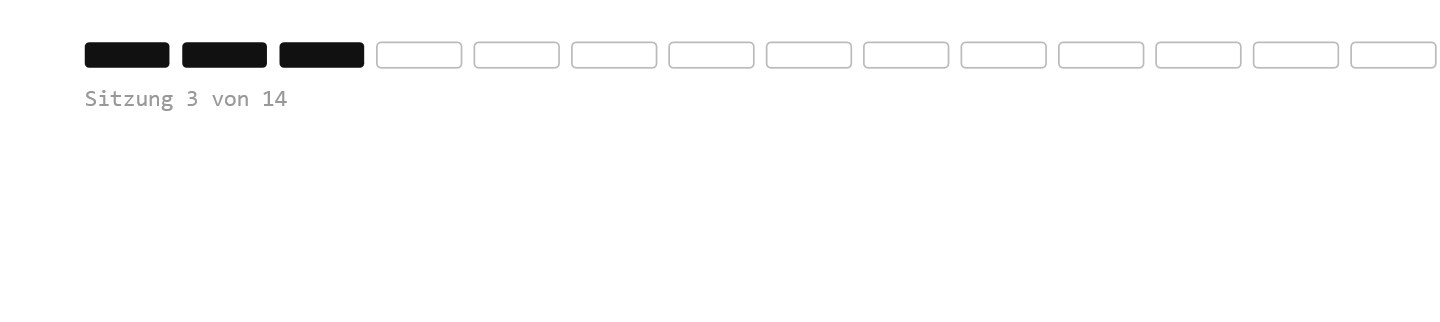
\includegraphics[keepaspectratio]{images/clipboard-3542587166.png}}

\pandocbounded{\includegraphics[keepaspectratio]{.pdf}}

\pandocbounded{
\includegraphics[keepaspectratio]{images/clipboard-2636932712.png}}

\textbf{Übung 2} zu ``Data Wrangling'' bis spätestens Sonntagabend!

:::::::




\end{document}
